\subsection{Termómetros}

\par 
El termómetro es un instrumento de medición de temperatura. Desde su invención ha evolucionado mucho, principalmente a partir del desarrollo de los termómetros electrónicos digitales. La manera como un termómetro determina la temperatura dependera del tipo de termómetro que sea. 

\par \noindent
Inicialmente se fabricaron aprovechando el fenómeno de la dilatación, por lo que se prefería el uso de materiales con elevado coeficiente de dilatación, de modo que, al aumentar la temperatura, su estiramiento era fácilmente visible. La sustancia que se utilizaba más frecuentemente en este tipo de termómetros ha sido el mercurio, encerrado en un tubo de vidrio que incorporaba una escala graduada, pero también alcoholes coloreados en termómetros grandes.

\begin{figure}[H]
	\centering
	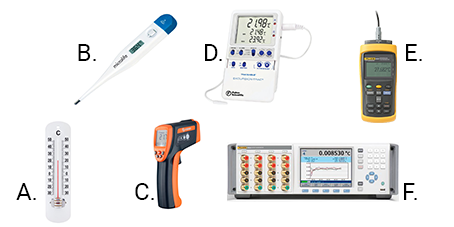
\includegraphics[width=\textwidth]{termometro1.png}
	\caption{Ejemplos de diferentes tipos de termómetros}
\end{figure}

\subsubsection{Escalas de temperatura}

\par 
La escala más usada en la mayoría de los países del mundo es la Celsius (\textdegree{}C) en honor a Anders Celsius (1701-1744) que se llamó centígrado hasta 1948. En esta escala, el cero (0 \textdegree{}C) y los cien (100 \textdegree{}C) grados corresponden respectivamente a los puntos de congelación y de ebullición del agua, ambos a la presión de 1 atmósfera.

\par \noindent 
Otras escalas termométricas son:

\begin{itemize}
	
\item Fahrenheit (\textdegree{}F) 

Propuesta por Daniel Gabriel Fahrenheit en la revista Philosophical Transactions (Londres, 33, 78, 1724). El grado Fahrenheit es la unidad de temperatura en el sistema anglosajón de unidades, utilizado principalmente en Estados Unidos.

\item Kelvin (K) o temperatura absoluta: 

Es la escala de temperatura del Sistema Internacional de Unidades. Aunque la magnitud de una unidad Kelvin (K) coincide con un grado Celsius (\textdegree{}C), el cero se ha fijado en el cero absoluto a -273,15 \textdegree{}C y es inalcanzable según el tercer principio de la termodinámica.
\end{itemize}

\subsubsection{Tipos de termómetros}

\begin{itemize}
	\item Termómetro de mercurio: es un tubo de vidrio sellado que contiene mercurio, cuyo volumen cambia con la temperatura de manera uniforme. Este cambio de volumen se aprecia en una escala graduada. El termómetro de mercurio fue inventado por Gabriel Fahrenheit en el año 1714. Ver figura 2.14 (A)
	
	\item Pirómetros:  termómetros para altas temperaturas, se utilizan en fundiciones, fábricas de vidrio, hornos para cocción de cerámica, etc. Existen varios tipos según su principio de funcionamiento:
	
	\begin{itemize}
		
		\item Pirómetro óptico: se basan en la ley de Wien de distribución de la radiación térmica, según la cual, el color de la radiación varía con la temperatura. El color de la radiación de la superficie a medir se compara con el color emitido por un filamento que se ajusta con un reostato calibrado. Se utilizan para medir temperaturas elevadas, desde 700 °C hasta 3.200 °C, a las cuales se irradia suficiente energía en el espectro visible para permitir la medición óptica. Ver figura 2.14 (B)
		
	\end{itemize}
	
	\item Termómetro de lámina bimetálica: formado por dos láminas de metales de coeficientes de dilatación muy distintos y arrollados dejando el coeficiente más alto en el interior. Se utiliza sobre todo como sensor de temperatura en el termohigrógrafo.
	
	\begin{figure}[H]
		\centering
		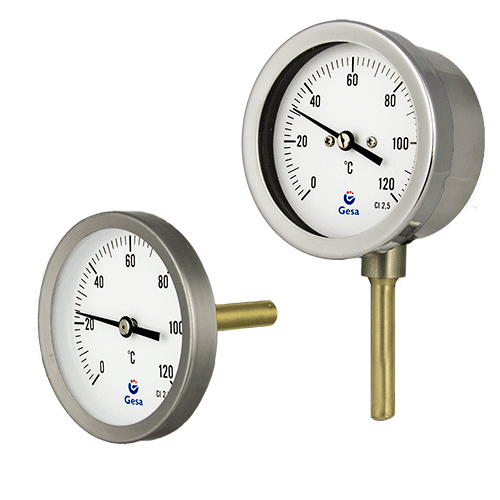
\includegraphics[width=5cm, height=5cm]{termometro2.png}
		\caption{Ejemplo de termómetro de lámina bimetálica}
	\end{figure}
	
	\clearpage
	
	\item Termómetro de gas: pueden ser a presión constante o a volumen constante. Este tipo de termómetros son muy exactos y generalmente son utilizados para la calibración de otros termómetros.
	
	\begin{figure}[H]
		\centering
		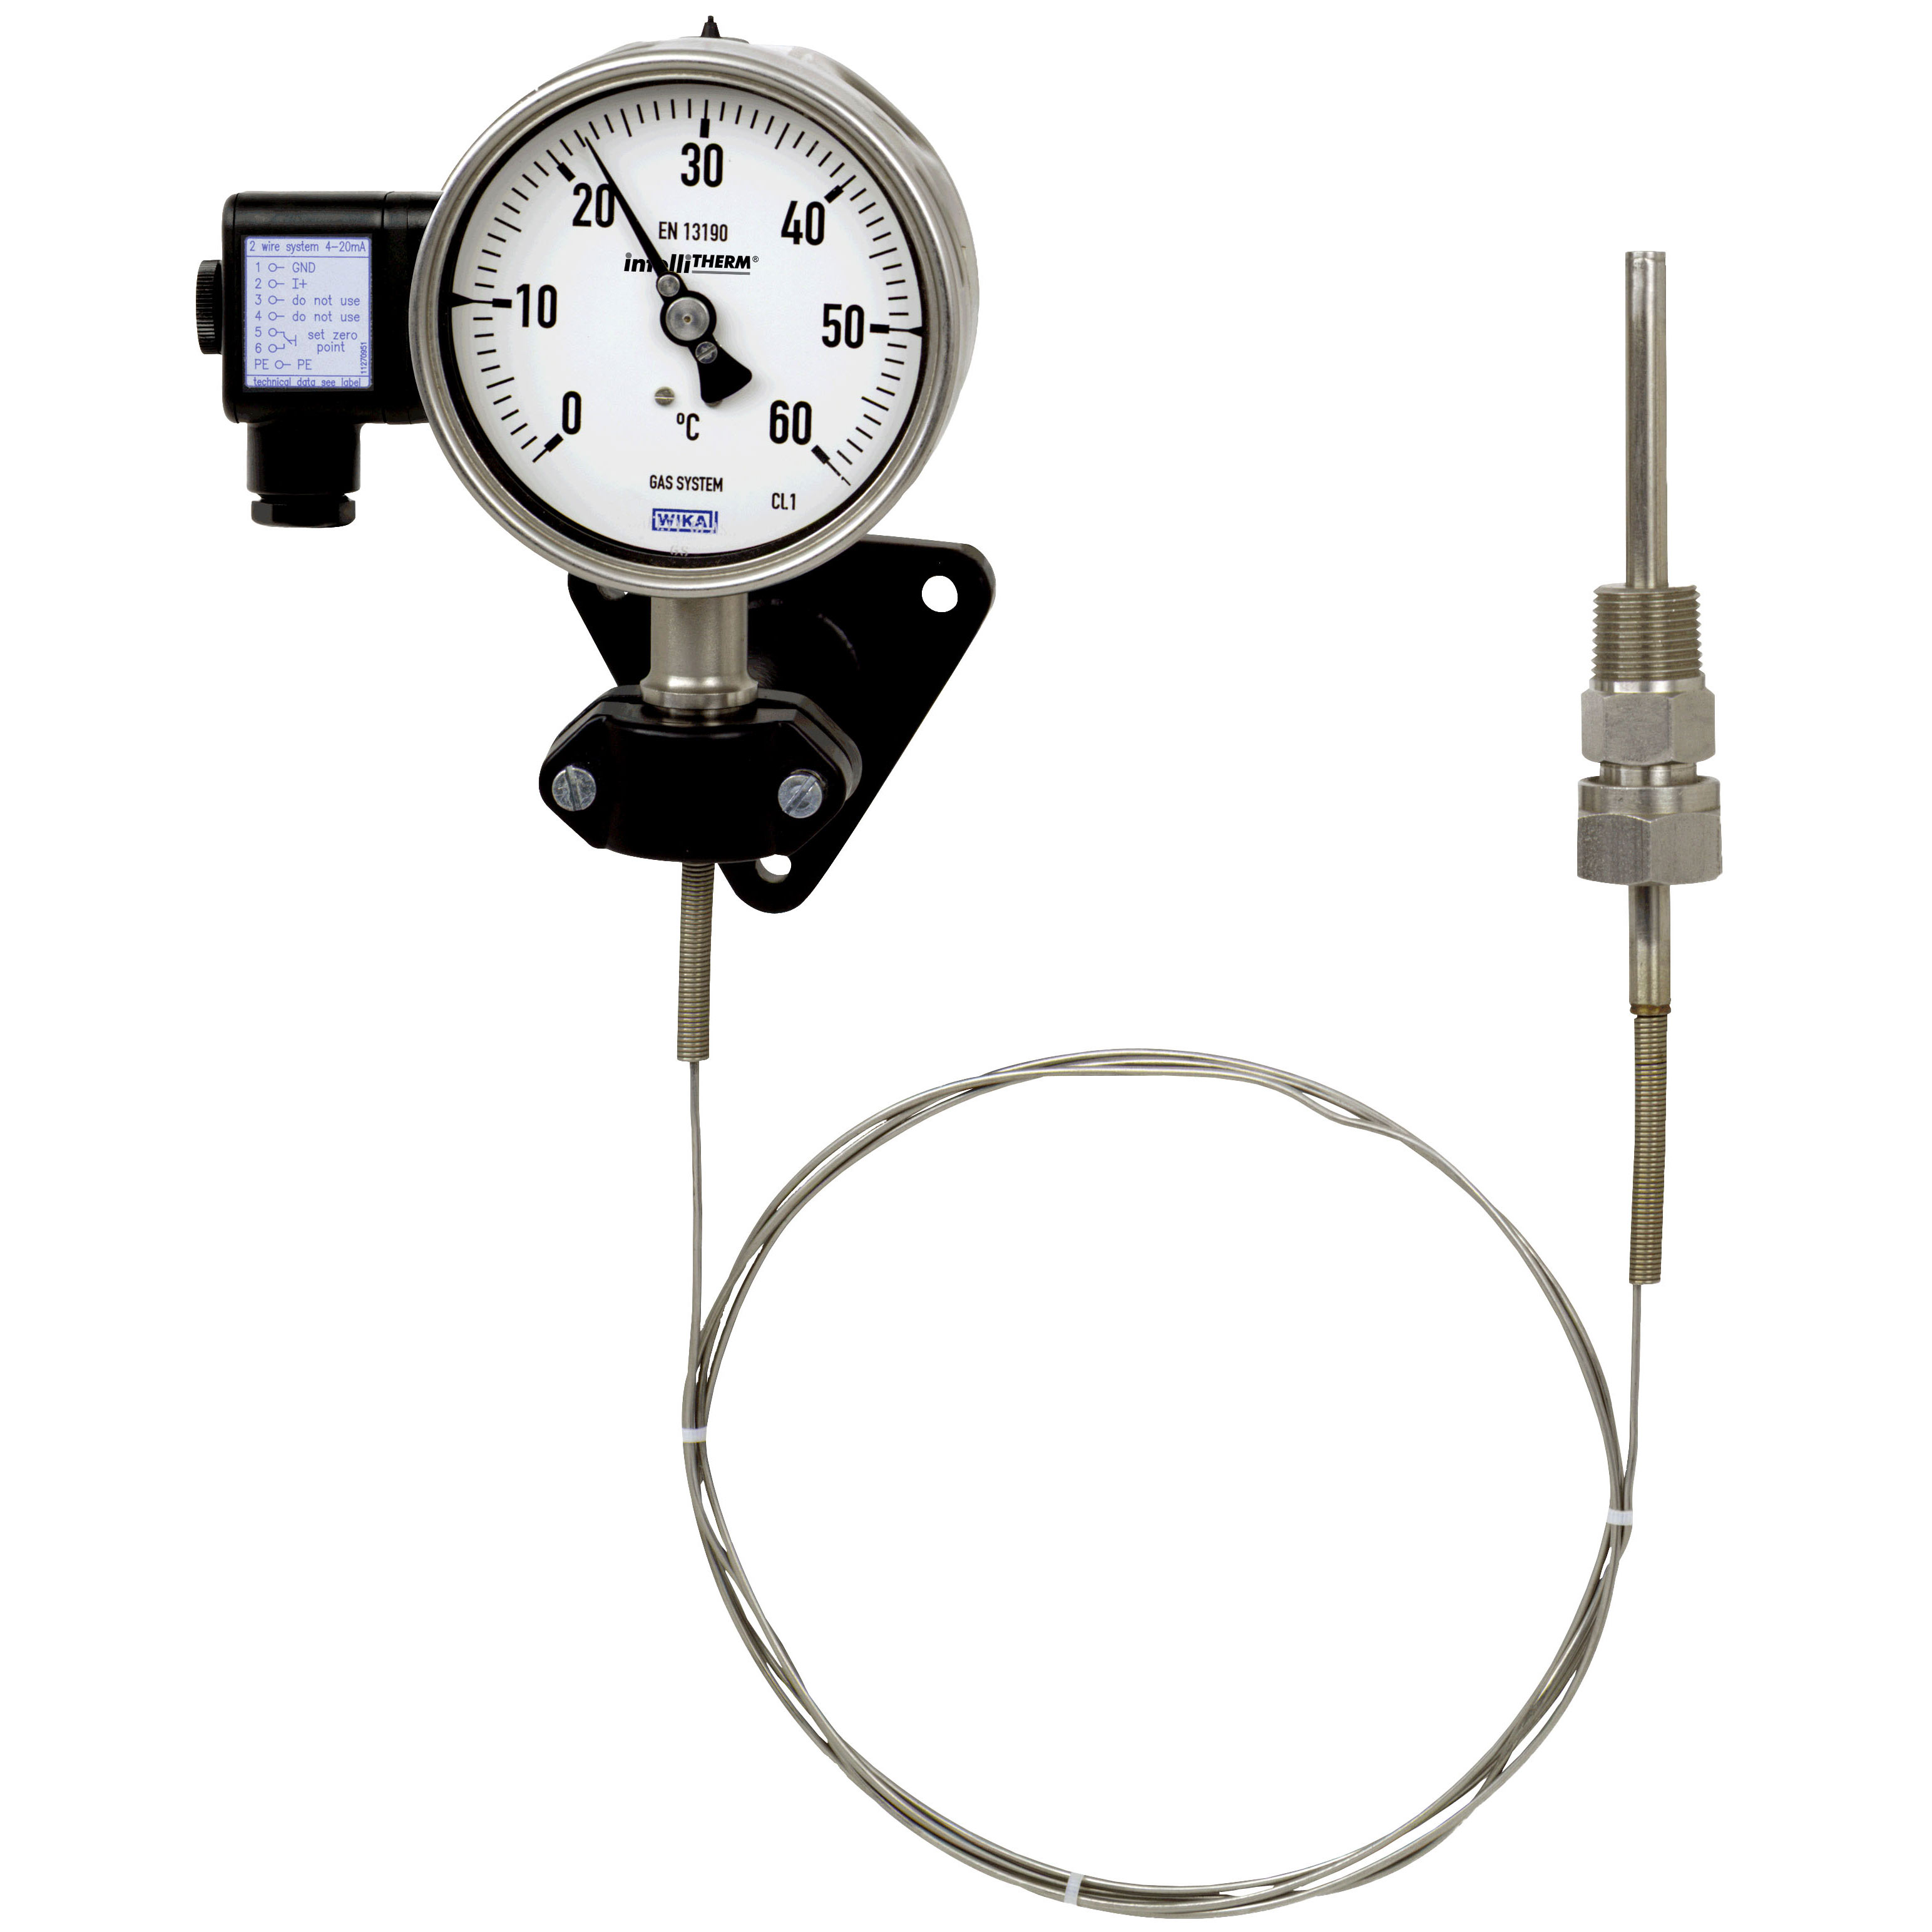
\includegraphics[width=4cm, height=4cm]{termometro3.jpg}
		\caption{Ejemplo de termómetro de gas}
	\end{figure}
	
	\item Termómetros digitales: son aquellos que, valiéndose de dispositivos transductores, utilizan luego circuitos electrónicos para convertir en números las pequeñas variaciones de tensión obtenidas, mostrando finalmente la temperatura en un visualizador. Una de sus principales ventajas es que por no utilizar mercurio no contaminan el medio ambiente cuando son desechados. Los dispositivos visualizadores pueden ser:
	
	\begin{itemize}
		
		\item Resistencia de platino: consiste en un alambre de algún metal de platino cuya resistencia eléctrica cambia cuando varía la temperatura. Van conectados a un termómetro digital como en la figura 2.14 (D, E y F)
		
		\item Termopar: Tambien conocido comoo termocupla es un dispositivo utilizado para medir temperaturas basado en la fuerza electromotriz que se genera al calentar la soldadura de dos metales distintos. Van conectados a un termómetro digital como en la figura 2.14 (D y E)
		
		\item Termistor:  es un dispositivo que varía su resistencia eléctrica en función de la temperatura. Algunos termómetros hacen uso de circuitos integrados que contienen un termistor, como el LM35. Van conectados a un termómetro digital como en la figura 2.14 (D y E)
		
	\end{itemize}
	
	\item Termómetros clinicos: son los utilizados para medir la temperatura corporal. Los hay tradicionales de mercurio y digitales, teniendo estos últimos algunas ventajas adicionales como su fácil lectura, respuesta rápida, memoria y en algunos modelos alarma vibrante. Ver figura 2.14 (B)
	
	\item Termógrafo: El termógrafo es un termómetro acoplado a un dispositivo capaz de registrar, gráfica o digitalmente, la temperatura medida en forma continua o a intervalos de tiempo determinado. En la figura 2.14 (F) las mediciones van acompañadas de una grafica.
	
\end{itemize}
